\section{Intro}
\subsection{Goal}
\frame{%
   \frametitle{\subsecname}
   \framesubtitle{MC}
   MC is a functional, declarative language.
}
\frame{%
   \frametitle{\subsecname}
   \framesubtitle{Why MC}
   Complexity compiler Casanova\\
   MC is the solution
}
\frame{%
   \frametitle{\subsecname}
   \framesubtitle{Goal of MC}
   MC adds abstraction\\
   \begin{itemize}
      \item Implementing compiler Casanova
      \item Teaching
   \end{itemize}
}

\subsection{MC basics}

\begin{frame}[fragile]
   \frametitle{\subsecname}
   \framesubtitle{Func}

   Creates a runtime function\\
   Premise, bar, rule
   \begin{lstlisting}
Func "foo" -> Bool -> Int -> Int -> Int

add b c -> res
---------------
foo True b c -> res

mul b c -> res
---------------
foo False b c -> res
   \end{lstlisting}
\end{frame}

\begin{frame}[fragile]
   \frametitle{\subsecname}
   \framesubtitle{Data}

   Constructs and Deconstructs types
   \begin{lstlisting}
Data "Left"  -> string -> string | float
Data "Right" -> float  -> string | float
   \end{lstlisting}
\end{frame}

\begin{frame}[fragile]
   \frametitle{\subsecname}
   \framesubtitle{TypeFunc}

   Creates a compile time function and is able to create kinds
   \begin{lstlisting}
TypeFunc "bar" => * => *

a => (c * d)
(d * c) => res
---------------
bar a => res
   \end{lstlisting}
\end{frame}

\begin{frame}[fragile]
   \frametitle{\subsecname}
   \framesubtitle{TypeAlias}

   The same as Data
   Constructs and Deconstructs kinds
\end{frame}

\begin{frame}[fragile]
   \frametitle{\subsecname}
   \framesubtitle{Module}

   Defines an interface
   \begin{lstlisting}
TypeFunc "MonoidAdd" => #a => Module
MonoidAdd 'a => Module {
  Func 'a -> "+" -> 'a -> 'a
  Func "identityAdd" -> 'a
}
   \end{lstlisting}
\end{frame}

\section{MC standardlibrary}
\subsection{Monad Transformers}
\subsubsection{Monads}
% \frame{%
% explain mathematical
% endofunctors
% monoid
% }
\frame{%
   \frametitle{\subsecname}
   \framesubtitle{\subsubsecname}

   \begin{itemize}
      \item Monads
         \begin{itemize}
            \item Generic interface
            \item Container-like
            \item Two functions
         \end{itemize}
   \end{itemize}
}

\frame{%
   \frametitle{\subsecname}
   \framesubtitle{\subsubsecname}
   The return function

   \begin{figure}
      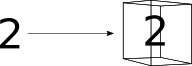
\includegraphics[width=\textwidth]{return}
   \end{figure}
}

\frame{%
   \frametitle{\subsecname}
   \framesubtitle{\subsubsecname}
   The bind function\\
   Step 1

   \begin{figure}
      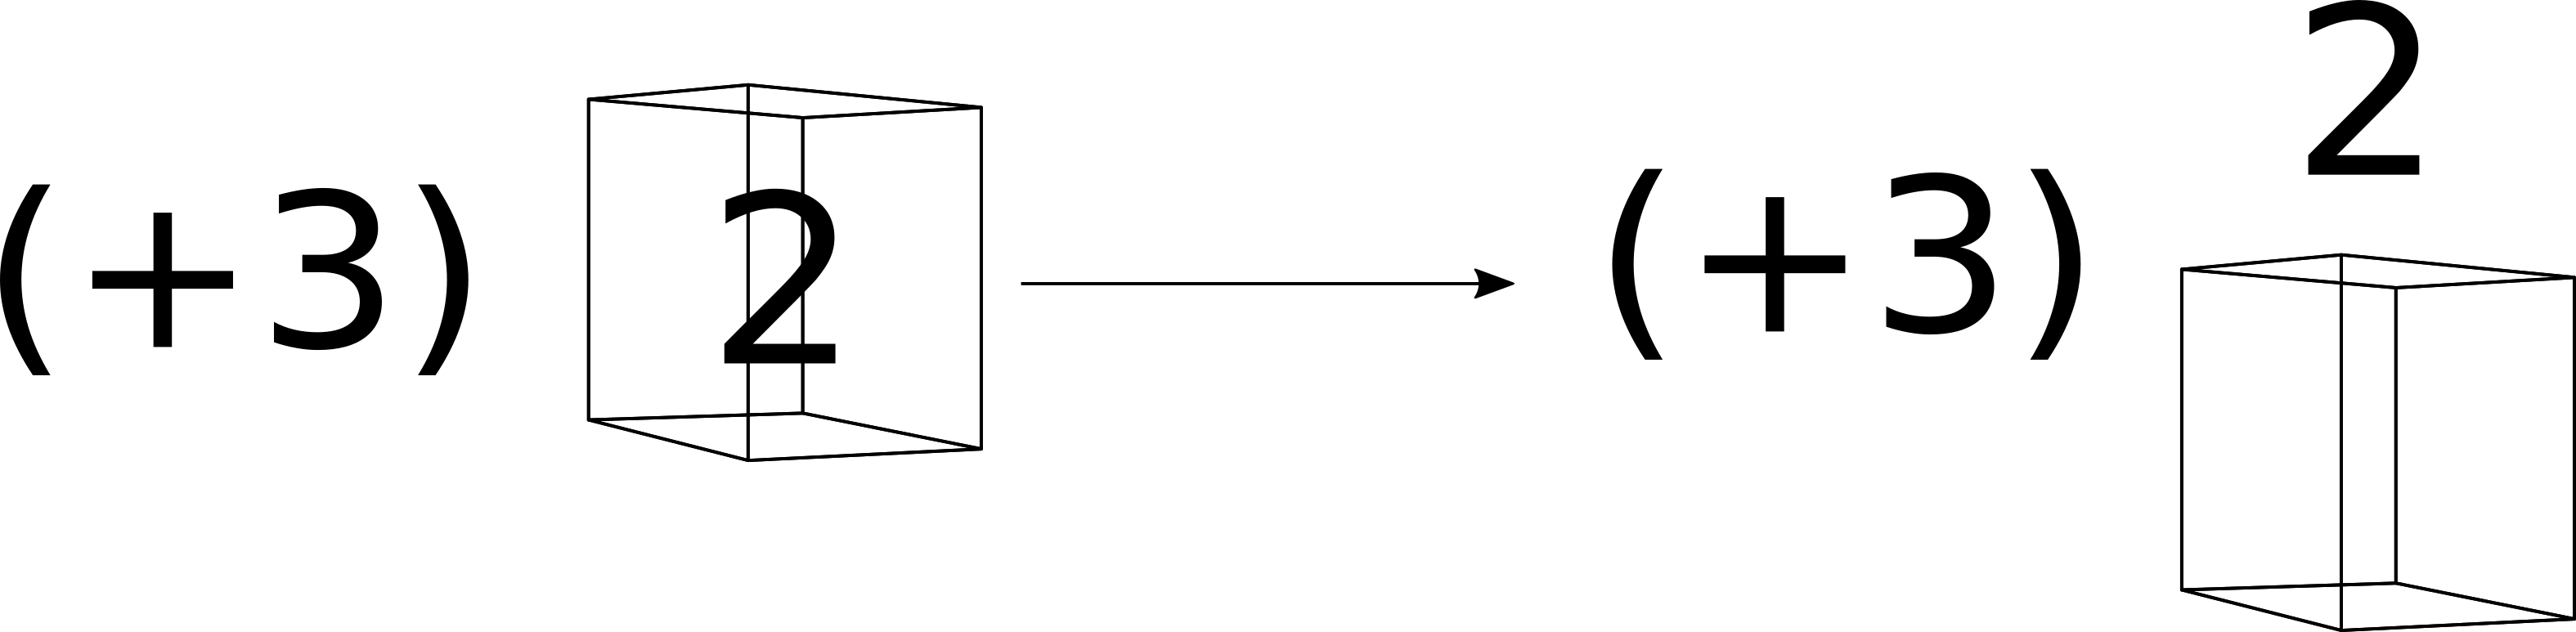
\includegraphics[width=\textwidth]{bind1}
   \end{figure}
}

\frame{%
   \frametitle{\subsecname}
   \framesubtitle{\subsubsecname}
   The bind function\\
   Step 2

   \begin{figure}
      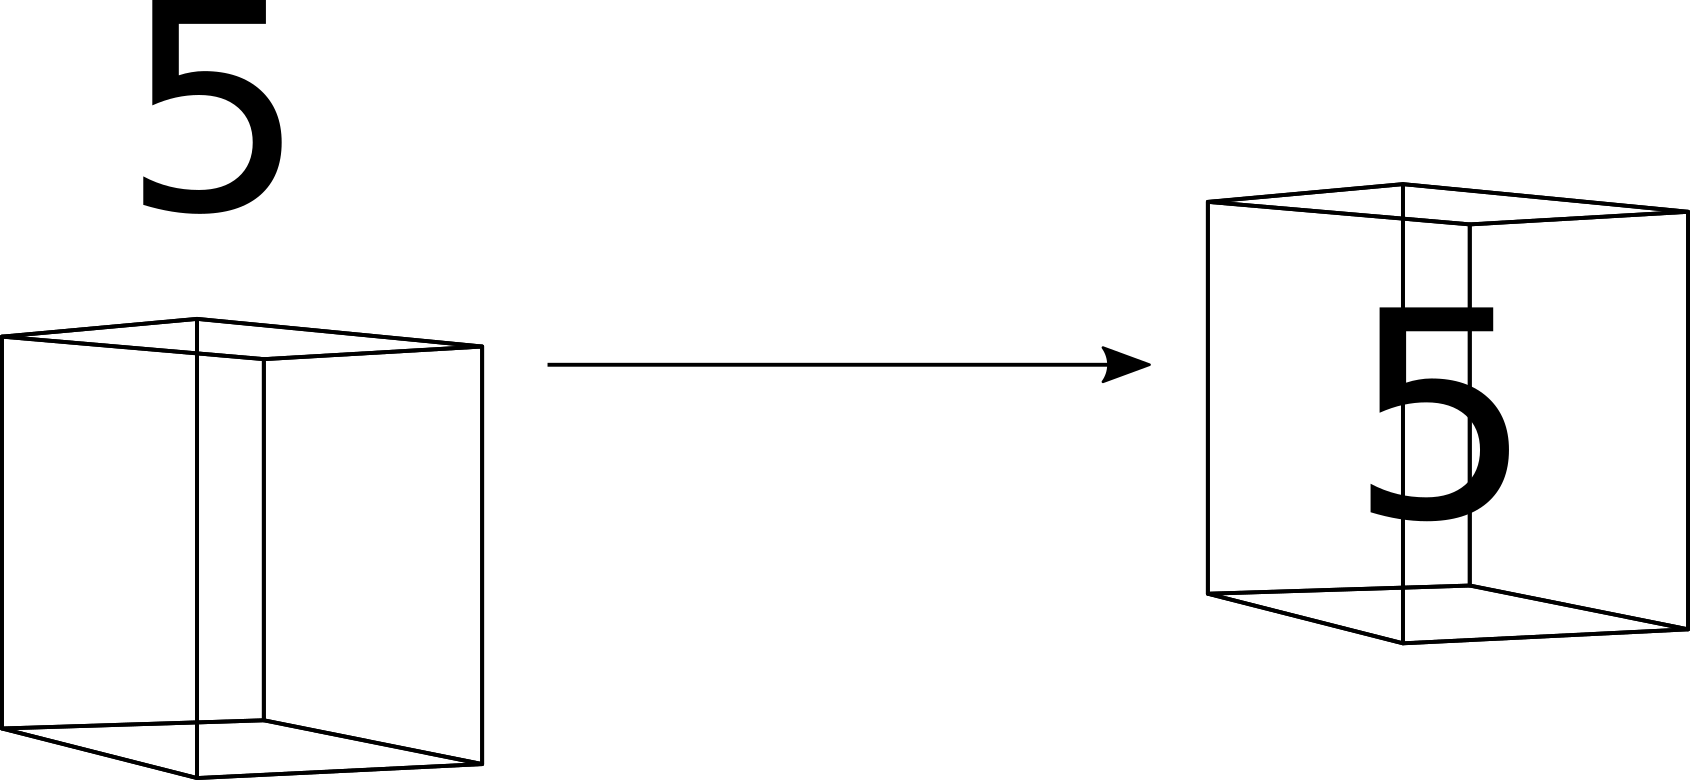
\includegraphics[width=\textwidth]{bind2}
   \end{figure}
}

\frame{%
   \frametitle{\subsecname}
   \framesubtitle{\subsubsecname}
   Different Monads
   \begin{itemize}
      \item State
      \item Maybe
   \end{itemize}
}

\frame{%
   \frametitle{\subsecname}
   \framesubtitle{\subsubsecname}

   Parser monad $\Longrightarrow$ State monad $\longrightarrow$ Maybe Monad \\
   \vspace{\baselineskip}

   Combining Monads:\\
   \begin{itemize}
      \item By hand
      \item Error prone
   \end{itemize}
}

\subsubsection{Transformers}
   \frame{%
   \frametitle{\subsecname}
   \framesubtitle{\subsubsecname}

   \begin{figure}
      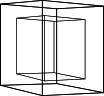
\includegraphics{transformers}
   \end{figure}

   \begin{itemize}
      \item Automatically combines monads
      \item Id monad
   \end{itemize}
}
\begin{frame}[fragile]
   \frametitle{\subsecname}
   \framesubtitle{\subsubsecname}
   Id monad
   \begin{lstlisting}
TypeAlias "Id" => #a => #b
Id 'a => 'a

TypeFunc "id" => Monad
id => Monad(Id) {
  bind x k -> k x
  return x -> x
}
   \end{lstlisting}
\end{frame}

\subsection{Records}
\frame{%
   \frametitle{\subsecname}
   \begin{itemize}
      \item Map or Key-Value list
      \item Inlined on Compile time
      \item Type safe
      \item Not built in
   \end{itemize}
}

\subsection{Updatables}
\frame{%
   \frametitle{\subsecname}

   \begin{itemize}
      \item Inlined on Compile time
      \item Functions
         \begin{itemize}
            \item Update
            \item Apply
         \end{itemize}
      \item Not built in
   \end{itemize}
}

\frame{%
   \frametitle{\subsecname}
   Consequences in use:
   \begin{itemize}
      \item Structure is bypassed
      \item Faster code
      \item Full power of mutables
   \end{itemize}
}

\subsection{Updatable Records}
\frame{%
   \frametitle{\subsecname}
   \begin{itemize}
      \item Inlined on Compile time
      \item Full power of mutable records
      \item State machine
   \end{itemize}

}
% \subsection{Coroutines}
% \frame{%
% \frametitle{\subsecname}

% }
